\chapter{Polymorphism and Traits}

When building complex software systems, we frequently encounter the need to represent diverse concepts that share common capabilities. For instance, in an e-commerce application, you might define distinct data structures to represent a \texttt{User} and an \texttt{Order}. While their internal memory layouts and business logic differ entirely, both might need to be ``validated'' before being processed or saved to a database. 

If we were to write entirely disjoint validation routines without a unifying abstraction, our codebase would quickly become repetitive and brittle. We need a way to express that different types can exhibit a shared behavior. In programming language theory, the ability to present the same interface for differing underlying forms is known as \textit{polymorphism}. 

\begin{notebox}
\textbf{The DRY Principle} \\
A core tenet of software engineering is DRY (Don't Repeat Yourself). Polymorphism is a fundamental tool for adhering to this principle, allowing us to write generalized code that seamlessly operates over a variety of concrete types.
\end{notebox}

In traditional programming paradigms, polymorphism is typically achieved through several distinct mechanisms. Object-oriented languages, such as Java or C++, heavily rely on classical \textbf{class inheritance} (subtyping polymorphism), where types descend from a common ancestor to inherit shared behavior. Alternatively, they use \textbf{interface programming} to define explicit contracts, or \textbf{generic programming} (parametric polymorphism) to write algorithms that operate on generic types without knowing their exact form ahead of time.

However, rigid object-oriented taxonomies based on inheritance often struggle to gracefully model the real world. In reality, behaviors cross-cut across completely unrelated types. 

\begin{insightbox}
\textbf{The Biology Taxonomy Analogy} \\
The professor highlighted how rigid inheritance hierarchies fall apart in complex domains, using biology as an example. Traditional taxonomy divides the world cleanly into Animals and Plants. But what about Fungi? They are neither perfectly animal nor vegetal, sitting awkwardly in the middle. Rigid object-oriented inheritance forces developers into these difficult classification decisions because types must fit strictly into a single tree.
\end{insightbox}

To avoid the pitfalls of rigid class hierarchies, Rust adopts a completely different approach based on \textbf{Traits}. Rust rejects classical inheritance entirely; instead, it separates the structural data (the \texttt{struct} or \texttt{enum}) from the behavior. By using traits to formalize shared behavior, Rust seamlessly combines the strengths of interface programming and generics. Types simply opt-in to a behavior by implementing a trait, allowing developers to model complex, cross-cutting capabilities without being forced into a restrictive inheritance tree.

\section*{Defining and Implementing Traits}

A Trait in Rust is essentially a contract. It declares a set of method signatures that a type must implement to satisfy that contract. The professor likened traits to interfaces in Java (such as \texttt{Runnable} or \texttt{Cloneable}), where a class commits to providing specific methods like \texttt{run()} or \texttt{clone()}. However, unlike Java, Rust traits are implemented without any inherent object hierarchy.

Let us build our intuition by modeling the validation scenario. We can define a \texttt{Validatable} trait that promises a single method:

\begin{lstlisting}[language=Rust]
trait Validatable {
    fn validate(&self) -> bool;
}
\end{lstlisting}

This trait acts as an interface. It does not contain data; it simply states that anything claiming to be \texttt{Validatable} must provide a \texttt{validate} method returning a boolean. Now, let us apply this behavior to two entirely different concrete types:

\begin{lstlisting}[language=Rust]
struct User {
    name: String,
    age: u8,
}

struct Order {
    total: f64,
}

impl Validatable for User {
    fn validate(&self) -> bool {
        !self.name.trim().is_empty() && self.age >= 18
    }
}

impl Validatable for Order {
    fn validate(&self) -> bool {
        self.total > 0.0
    }
}

struct PhoneNumber {
    number: String,
}

impl Validatable for PhoneNumber {
    fn validate(&self) -> bool {
        // Professor's domain rule: must start with '+' and have a maximum length
        self.number.starts_with('+') && self.number.len() <= 16
    }
}
\end{lstlisting}

This code effectively demonstrates how distinct types isolate their logic:
\begin{itemize}
    \item \textbf{Step 1:} We define a \texttt{PhoneNumber} containing simply a \texttt{String}.
    \item \textbf{Step 2:} We create an \texttt{impl Validatable for PhoneNumber} block, uniquely associating the trait's contract with this type.
    \item \textbf{Step 3:} We provide a custom implementation of \texttt{validate} that executes business logic specific to phone numbers (checking for a leading \texttt{+} and enforcing a length limit of 16 characters).
\end{itemize}

\textbf{Memory Model Analysis:} In this snippet, \texttt{User} contains a \texttt{String}, which is a heap-allocated buffer managed by a stack-allocated structure (pointer, capacity, length). The \texttt{age} field is an 8-bit integer allocated directly on the stack. When \texttt{validate(\&self)} is called, ownership of the \texttt{User} or \texttt{Order} is not transferred. Instead, an immutable borrow (\texttt{\&self}) is created. This allows the method to read the fields without consuming the instance, meaning the caller retains ownership. The lifetime of the borrow is strictly tied to the duration of the method call, guaranteeing no dangling pointers can occur while accessing the data.

Notice the syntax: \texttt{impl Validatable for User}. This block is entirely separate from the standard \texttt{impl User} block where we might define the struct's native methods. By isolating the trait implementation, we explicitly declare that the \texttt{validate} method is not just a coincidental name, but a fulfillment of the \texttt{Validatable} contract.

\begin{insightbox}
\textbf{Default Implementations} \\
Traits can also provide default implementations for their methods. If a trait defines a method body, the implementing type can choose to either use the provided default or override it with its own custom logic. This is highly useful for providing base functionality out of the box.
\end{insightbox}

One of the most powerful features of Rust's trait system is the ability to implement custom traits for types that you did not originally define, including types from the standard library. For example, we can make standard strings or integers implement our \texttt{Validatable} trait:

\begin{lstlisting}[language=Rust]
impl Validatable for String {
    fn validate(&self) -> bool {
        !self.trim().is_empty()
    }
}

impl Validatable for i32 {
    fn validate(&self) -> bool {
        *self > 0
    }
}
\end{lstlisting}

This allows developers to extend the behavior of built-in types to fit their specific domain logic seamlessly. However, to prevent conflicts, Rust enforces strict rules: you can only implement a trait for a type if either the trait or the type is defined within your current crate.

Once we have formalized this common behavior, we unlock the power of polymorphism. We can now write functions that operate not on specific structs, but on \textit{any} type that implements our trait. Rust provides two fundamental mechanisms to achieve this: \textbf{Static Dispatch} and \textbf{Dynamic Dispatch}.

\section*{Static Dispatch and Monomorphization}

The most common way to leverage traits is through generic programming. We can write a function that accepts any generic type \texttt{T}, but we constrain \texttt{T} using a trait bound:

\begin{lstlisting}[language=Rust]
fn check<T: Validatable>(item: &T) {
    if item.validate() {
        println!("The item is valid.");
    } else {
        println!("Validation failed!");
    }
}
\end{lstlisting}

Here, \texttt{<T: Validatable>} tells the compiler that this function accepts a reference to any type \texttt{T}, provided that \texttt{T} implements \texttt{Validatable}. Because of this guarantee, the compiler allows us to safely call \texttt{item.validate()} inside the function body. 

If a generic type must satisfy multiple behaviors, we can combine trait bounds using the \texttt{+} operator. For functions with complex signatures, Rust provides the \texttt{where} clause to keep the function declaration clean and readable:

\begin{lstlisting}[language=Rust]
// Compact syntax for multiple bounds
fn process<T: Validatable + Clone>(item: &T) { /* ... */ }

// Extended syntax using 'where'
fn process_cleaner<T>(item: &T) 
where 
    T: Validatable + Clone 
{ 
    /* ... */ 
}
\end{lstlisting}

But how does this execute at the hardware level? Unlike languages like Java, which use Type Erasure and process generic types as opaque objects at runtime, Rust uses a mechanism called \textbf{Monomorphization}.

When the Rust compiler sees calls to the \texttt{check} function---perhaps once with a \texttt{User} and once with an \texttt{Order}---it acts as a code generator. It creates two entirely separate, specialized copies of the \texttt{check} function:

\begin{lstlisting}[language=Rust]
// Generated internally by the compiler
fn check_user(item: &User) { /* static call to User::validate */ }
fn check_order(item: &Order) { /* static call to Order::validate */ }
\end{lstlisting}

Because the compiler generates specialized machine code for every type used, the CPU executes a direct static call to the specific \texttt{validate} method. There is zero runtime overhead. 

\begin{insightbox}
\textbf{Rust Monomorphization vs. Java Type Erasure} \\
The professor explicitly contrasted Rust's approach with Java's generic programming. In Java, generic lists like \texttt{ArrayList<T>} use a mechanism called \textit{Type Erasure}. Java does not generate a specialized list for strings and another for integers; it compiles a single generic list that operates on raw \texttt{Object} references. This minimizes code duplication but sacrifices performance, as it necessitates dynamic method lookups and forces primitive types (like \texttt{int}) to be boxed into objects (like \texttt{Integer}). Rust's Monomorphization does the exact opposite: it duplicates the code for each type, avoiding object boxing and maximizing CPU performance at the cost of slightly larger binaries.
\end{insightbox}

\begin{examprioritybox}
\textbf{Static Dispatch vs. Dynamic Dispatch: The Embedded vs. High-Frequency Trade-off} \\
The professor heavily emphasizes the contrasting architectural impacts of these two mechanisms. Monomorphization (Static Dispatch) duplicates code for every concrete type used. While this enables aggressive compiler optimizations (like inlining) and zero-cost runtime abstraction, it causes \textit{code bloat}. This is critically problematic in embedded systems (e.g., microcontrollers like the Atmel 328 with just 2KB of RAM) where binary size is strictly constrained. Conversely, Dynamic Dispatch uses a single function copy and resolves methods at runtime via Fat Pointers and VTables, saving space but incurring CPU cycles for pointer indirection. This micro-delay is unacceptable in scenarios where every CPU cycle translates to massive scale, such as High-Frequency Trading, intensive LLM (Large Language Model) training, or Bitcoin mining hashing algorithms.

\textbf{Common Pitfall:} Assuming one dispatch method is universally superior. Overusing static generics in memory-constrained environments can lead to compilation failures due to binary size limits, whereas overusing dynamic dispatch can silently degrade performance in tight computational loops. \\
\textbf{Expected Mastery Level:} High. You must be able to confidently justify when to use \texttt{<T: Trait>} versus \texttt{\&dyn Trait} based on specific hardware or performance constraints.
\end{examprioritybox}

\section*{Dynamic Dispatch and Trait Objects}

While static dispatch is fast, it is not always flexible enough. Because monomorphization requires generating distinct functions, you cannot, for example, easily store a mix of \texttt{User} and \texttt{Order} objects in a single vector, since a \texttt{Vec<T>} strictly requires all elements to be of the exact same compile-time type \texttt{T}.

When we need a truly heterogeneous collection or want to avoid code duplication entirely, we use \textbf{Dynamic Dispatch}. In Rust, dynamic dispatch is achieved using \textit{Trait Objects}, denoted by the \texttt{dyn} keyword.

\begin{lstlisting}[language=Rust]
fn check_dynamic(item: &dyn Validatable) {
    if item.validate() {
        println!("The item is valid.");
    }
}
\end{lstlisting}

\textbf{Memory Model Analysis:} When passing a reference to \texttt{check\_dynamic(item: \&dyn Validatable)}, the standard reference is implicitly converted into a Fat Pointer on the stack. This Fat Pointer consists of two machine words: a data pointer referencing the actual instance (which may live on the stack or heap) and a VTable pointer referencing a statically allocated virtual method table. The VTable itself resides in the read-only data segment of the compiled binary. No ownership is transferred during this dynamic call; the borrow checker statically ensures that the underlying data outlives the Fat Pointer.

Instead of generating specialized copies, the compiler creates only \textit{one} version of the \texttt{check\_dynamic} function. This single function is capable of handling any type that implements \texttt{Validatable}. However, because the compiler does not know the specific size or type of the data at compile time, it must resolve the correct method to call at runtime.

\subsection*{The Mechanism: Fat Pointers and VTables}

To make runtime method resolution possible, the reference \texttt{\&dyn Validatable} is not a standard pointer; it is a \textbf{Fat Pointer}. A fat pointer occupies twice the size of a standard system pointer because it actually consists of two separate pointers packed together:

\begin{enumerate}
    \item \textbf{Data Pointer}: Points to the actual instance in memory (e.g., the specific \texttt{User} or \texttt{Order} struct).
    \item \textbf{VTable Pointer}: Points to a static Virtual Method Table (\texttt{vtable}) constructed specifically for that concrete type during compilation.
\end{enumerate}

\begin{figure}[h]
    \centering
    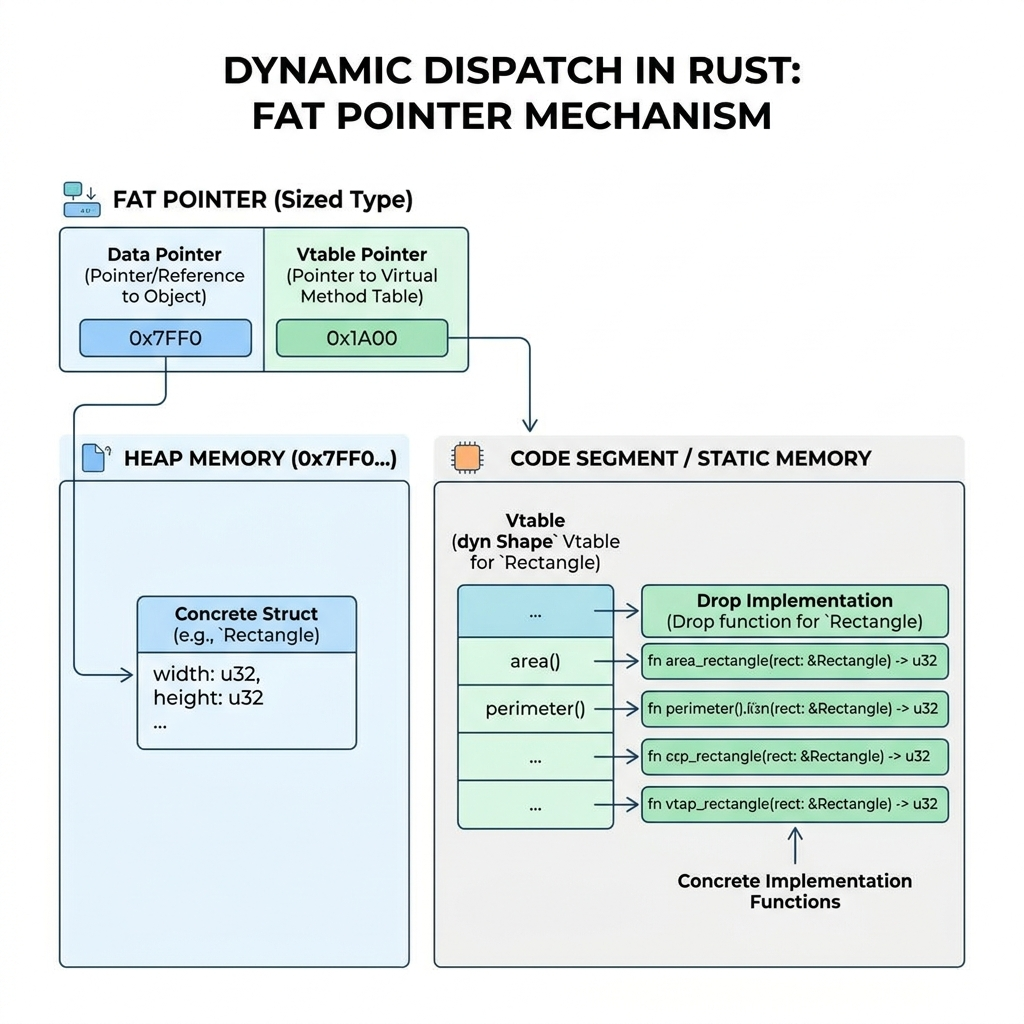
\includegraphics[width=0.8\textwidth]{images/vtable.png}
    \caption{Memory layout of a Trait Object representing a Fat Pointer and its corresponding VTable.}
    \label{fig:vtable}
\end{figure}

As visualized in Figure \ref{fig:vtable}, the \texttt{vtable} is an array of function pointers. It contains metadata about the type (like its size and memory alignment, which are required to run the destructor via \texttt{drop}), followed by pointers to the specific implementations of the trait's methods. 

When \texttt{item.validate()} is called inside \texttt{check\_dynamic}, the program dereferences the fat pointer, navigates to the \texttt{vtable}, finds the index corresponding to the \texttt{validate} function, and finally jumps to that code segment, passing the data pointer as \texttt{\&self}.

\begin{exambox}
\textbf{Trade-offs of Dynamic Dispatch} \\
Dynamic dispatch yields a smaller binary footprint because it does not duplicate code. It also allows for heterogeneous collections, such as a \texttt{Vec<Box<dyn Validatable>>}. The penalty is runtime overhead: looking up the function in the \texttt{vtable} requires extra memory jumps (pointer indirection), which is less cache-friendly and prevents compiler optimizations like inlining. While the cost is measured in nanoseconds, it becomes highly relevant in high-frequency trading or intensive numerical simulations.
\end{exambox}

\begin{warningbox}
\textbf{Object Safety Limits} \\
Not all traits can be turned into Trait Objects via \texttt{dyn}. A trait must be \textit{Object Safe}. The two primary rules are:
1. The trait's methods must not return \texttt{Self} (since the compiler wouldn't know the size of the returned object dynamically at compile time).
2. The methods must not have generic type parameters.
If a trait violates these rules, the compiler will safely refuse to create a \texttt{dyn Trait} fat pointer for it.
\end{warningbox}

\section*{Advanced Trait Patterns}

To write highly robust and expressive code, Rust provides additional constructs built on top of the base trait system. Two notable mechanisms are Associated Types and Supertraits.

\subsection*{Associated Types}
Sometimes, a trait needs to define a relationship with another type without forcing the implementer to specify generic parameters everywhere. We achieve this using an \textbf{Associated Type}.

\begin{lstlisting}[language=Rust]
trait Container {
    type Item; // Associated type
    
    fn get(&self) -> &Self::Item;
}

struct IntBox {
    value: i32,
}

impl Container for IntBox {
    type Item = i32; // Concrete specification
    
    fn get(&self) -> &i32 {
        &self.value
    }
}
\end{lstlisting}

By declaring \texttt{type Item;}, we dictate that whoever implements \texttt{Container} must explicitly define what \texttt{Item} is. This is heavily used in standard library traits, most notably \texttt{Iterator}, which defines \texttt{type Item} to indicate the type of element the iterator will yield. 

To demonstrate how traits and generics can elegantly combine, the professor showed that \texttt{Container} can also be implemented for a generic struct:

\begin{lstlisting}[language=Rust]
struct Boxed<T> {
    value: T,
}

impl<T> Container for Boxed<T> {
    type Item = T; // The associated type dynamically maps to the generic parameter
    
    fn get(&self) -> &T {
        &self.value
    }
}
\end{lstlisting}

Here is how generics integrate with associated types step-by-step:
\begin{itemize}
    \item \textbf{Step 1:} A struct \texttt{Boxed<T>} is defined to generically hold any type \texttt{T}.
    \item \textbf{Step 2:} When implementing the \texttt{Container} trait, we declare \texttt{impl<T> Container for Boxed<T>}, bringing the generic parameter into the trait implementation's scope.
    \item \textbf{Step 3:} We explicitly map the trait's associated type \texttt{Item} to the generic parameter \texttt{T}. This tells the compiler that the returned type of \texttt{get} will always match the type stored in the box.
\end{itemize}

While you could achieve somewhat similar functionality using a generic trait like \texttt{trait Container<T>}, associated types drastically improve readability and prevent the complexity of managing multiple overlapping generic implementations for a single struct.

\subsection*{Supertraits}
Often, one trait builds logically upon another. If a type wishes to implement a sophisticated trait, it must first prove it implements a foundational one. We define this dependency using a \textbf{Supertrait}.

\begin{lstlisting}[language=Rust]
trait Printable {
    fn print(&self);
}

// AdvancedPrintable requires Printable
trait AdvancedPrintable: Printable {
    fn print_twice(&self) {
        self.print();
        self.print();
    }
}
\end{lstlisting}

Here, \texttt{Printable} is a supertrait of \texttt{AdvancedPrintable}. The compiler enforces that any type attempting to implement \texttt{AdvancedPrintable} must also provide an implementation for \texttt{Printable}. This guarantees that methods relying on the foundational behavior (such as calling \texttt{self.print()} within \texttt{print\_twice()}) will always execute safely.

\section*{Standard Library Traits}

A significant portion of Rust's syntax and behavior is powered by traits defined in the standard library. Implementing these traits for your own types allows them to interact seamlessly with Rust's built-in operators and language features. For many of these, Rust can automatically generate the implementation using the \texttt{\#[derive(...)]} macro.

\subsection*{Comparison: \texttt{PartialEq}, \texttt{Eq}, \texttt{PartialOrd}, and \texttt{Ord}}
Rust separates equality and ordering into distinct traits to handle mathematical edge cases accurately.
\begin{itemize}
    \item \textbf{\texttt{PartialEq}}: Enables the use of the \texttt{==} and \texttt{!=} operators. It is ``partial'' because it allows for values that cannot be strictly compared to themselves (e.g., \texttt{NaN} in floating-point numbers where \texttt{NaN == NaN} is false). The professor highlighted a classic floating-point pitfall: checking \texttt{0.1 + 0.2 == 0.3} will yield \texttt{false} (it evaluates to \texttt{0.30000000000000004}). Because $0.1$ is a periodic number in base-2, it suffers from unavoidable rounding errors. Exact equality on floats is thus inherently unreliable, which is exactly why Rust uses \texttt{PartialEq} rather than total \texttt{Eq} for floating-point types.
    \item \textbf{\texttt{Eq}}: A marker trait that extends \texttt{PartialEq} to indicate a total equivalence relation (every value is strictly equal to itself).
    \item \textbf{\texttt{PartialOrd} and \texttt{Ord}}: Enable the use of relational operators (\texttt{<}, \texttt{>}, \texttt{<=}, \texttt{>=}). Similarly to equality, \texttt{PartialOrd} is for types where some values might not be comparable, whereas \texttt{Ord} defines a strict total order.
\end{itemize}

\subsection*{Formatting: \texttt{Display} and \texttt{Debug}}
To convert types into text, Rust uses two primary formatting traits:
\begin{itemize}
    \item \textbf{\texttt{Display}}: Designed for user-facing output (used with the \texttt{\{\}} format specifier). It must be implemented manually, as the programmer needs to define the specific representation suitable for end users.
    \item \textbf{\texttt{Debug}}: Intended for developer-facing output, providing an internal representation of the data (used with the \texttt{\{:?\}} format specifier). It can be automatically implemented via \texttt{\#[derive(Debug)]}.
\end{itemize}

\subsection*{Duplication: \texttt{Clone} vs. \texttt{Copy}}
When assigning a value to a new variable or passing it to a function, Rust's default behavior is to \textit{move} the value, transferring ownership.
\begin{itemize}
    \item \textbf{\texttt{Clone}}: Explicitly creates a duplicate of a value. Because cloning can involve expensive operations like heap allocations, it must be invoked explicitly via the \texttt{.clone()} method.
    \item \textbf{\texttt{Copy}}: A subtrait of \texttt{Clone} that changes the default assignment semantics from a \textit{move} to a \textit{copy}. It indicates that duplicating the value is simply a matter of copying bits, which is fast and cannot fail (e.g., primitive integers). It can only be implemented if all fields of the type also implement \texttt{Copy}.
\end{itemize}

\subsection*{Resource Management: \texttt{Drop}}
The \texttt{Drop} trait serves as Rust's equivalent of a destructor. It allows you to specify custom code that runs automatically when a value goes out of scope, releasing resources such as heap memory, network connections, or file handles (an implementation of the RAII pattern). 
If a programmer wishes to destroy a value prematurely, they can pass it to the globally available \texttt{std::mem::drop} function, forcing the value to be moved and subsequently destroyed.

\begin{memoryblock}
\textbf{The Mechanics of \texttt{std::mem::drop} and Container Destruction} \\
The professor clarified that \texttt{std::mem::drop(x)} is actually a deceivingly simple, entirely empty function: \texttt{fn drop<T>(\_x: T) \{\}}. By passing a variable into it by value, ownership of the data is transferred to the function's scope. Because the function ends immediately doing nothing, the variable goes out of scope and its \texttt{Drop} implementation is triggered early. \\
Furthermore, when a complex data structure like a \texttt{Vec<T>} goes out of scope, its \texttt{Drop} implementation traverses the collection, guaranteeing that the \texttt{drop} method is called sequentially on every single item it contains before the vector's own backing memory is finally released.
\end{memoryblock}

\begin{examprioritybox}
\textbf{Drop and Copy Mutual Exclusivity} \\
The professor heavily stressed that \texttt{Drop} and \texttt{Copy} are mutually exclusive. If a type implements \texttt{Drop}, it is actively managing a resource (e.g., a heap allocation or file handle). If such a type were allowed to be implicitly bit-wise copied via the \texttt{Copy} trait, you would end up with two instances holding pointers to the exact same underlying resource. When both instances go out of scope, the \texttt{drop} method would run twice, leading to catastrophic double-free vulnerabilities or resource corruption.

\textbf{Common Pitfall:} Trying to derive \texttt{Copy} on a struct that contains a heap-allocated field (like \texttt{String} or \texttt{Vec}) or a custom \texttt{Drop} implementation. The compiler will reject this immediately. \\
\textbf{Expected Mastery Level:} Very High. Understanding why \texttt{Drop} and \texttt{Copy} conflict is fundamental to grasping Rust's memory safety guarantees.
\end{examprioritybox}

\subsection*{Type Conversions: \texttt{From}, \texttt{Into}, and \texttt{FromStr}}
Rust prefers explicit type conversions. The \texttt{From} and \texttt{Into} traits define how to consume a value of one type to create a value of another. They are perfectly dual: implementing \texttt{From<T> for U} automatically provides an \texttt{Into<U>} implementation for \texttt{T}. However, conversion is not necessarily symmetric; being able to convert a \texttt{String} into a custom type does not automatically mean the reverse is possible or logical.

For parsing strings specifically, Rust offers the \texttt{FromStr} trait. Implementing it unlocks the ability to use the \texttt{.parse()} method on strings to instantiate your type, gracefully handling potential parsing failures by returning a \texttt{Result}. During the lecture, the professor gave the example of parsing a string into a custom struct by inspecting character slices, leveraging methods like \texttt{s.starts\_with()} and \texttt{s.trim()} inside the custom \texttt{from\_str} implementation.

\subsection*{Exam Relevance and Recurrence}
\textbf{Exam Relevance Score:} Very High \\
\textbf{Notes:} Questions on polymorphism in Rust appear frequently in exams, particularly concerning the architectural trade-offs between Monomorphization (Static Dispatch) and Trait Objects (Dynamic Dispatch). You are highly likely to be asked to compare the memory implications of both (code bloat vs. VTable lookup overhead). The structure and content of a Fat Pointer (data pointer + VTable pointer) is another recurring theoretical question. Furthermore, the mutual exclusivity of \texttt{Drop} and \texttt{Copy} traits is a classic exam topic used to test understanding of RAII and memory safety.

\section{Domande ed Esercizi da Esami Passati}

\begin{exambox}
\textbf{Domanda 1:} Nel contesto della programmazione generica, si spieghi che cosa si intende per monomorfizzazione.
Si scriva una porzione di codice che mostri un esempio pratico in cui la monomorfizzazione viene applicata, spiegando perché tale esempio è rilevante.
Si indichino i principali punti di forza e i punti di debolezza di tale proprietà, facendo un raffronto rispetto agli approcci alla programmazione generica offerti da altri linguaggi di programmazione.

\textbf{Soluzione:}
La monomorfizzazione è il meccanismo con cui il compilatore Rust implementa la programmazione generica (Static Dispatch). Quando una funzione accetta parametri generici vincolati da un trait, il compilatore non crea una singola funzione generica (come accade in Java tramite \textit{Type Erasure}), ma genera internamente copie distinte e specializzate della funzione per ogni tipo concreto utilizzato nel sorgente.

\textbf{Esempio Pratico:}
\begin{lstlisting}[language=Rust]
trait Validatable { fn validate(&self) -> bool; }

fn check<T: Validatable>(item: &T) { item.validate(); }

struct User;
impl Validatable for User { fn validate(&self) -> bool { true } }

struct Order;
impl Validatable for Order { fn validate(&self) -> bool { false } }

fn main() {
    let user = User;
    let order = Order;
    check(&user);  // Il compilatore genera check_user
    check(&order); // Il compilatore genera check_order
}
\end{lstlisting}
L'esempio è rilevante perché dimostra che \texttt{check} a livello di linguaggio macchina viene espansa in copie distinte (\texttt{check\_user}, \texttt{check\_order}) che effettuano chiamate dirette e statiche ai rispettivi metodi, senza alcuna ambiguità o ricerca a runtime.

\textbf{Raffronto e pro/contro:}
Il principale punto di forza è la prestazione (Zero-Cost Abstraction): le chiamate statiche non hanno overhead a runtime e permettono ottimizzazioni spinte come l'inlining. Il punto di debolezza è il \textit{code bloat} (aumento della dimensione del binario), particolarmente critico in sistemi embedded con memoria limitata. Al contrario, l'approccio in Java (Type Erasure) minimizza la duplicazione del codice utilizzando riferimenti a un generico \texttt{Object}, ma sacrifica le prestazioni necessitando di \textit{boxing} per i tipi primitivi e lookup dinamici a runtime.
\end{exambox}

\begin{exambox}
\textbf{Domanda 2:} Dato il seguente programma si descriva il comportamento del programma e la mappa della memoria utilizzata dalle variabili
\begin{lstlisting}[language=Rust]
1 fn main() {
2 trait Calculate {
3 fn add(&self, l: u64, r: u64) -> u64;
4 fn mul(&self, l: u64, r: u64) -> u64;
5 }
6 struct Modulo(u64);
\end{lstlisting}

\textbf{Soluzione:}
Il programma definisce un trait `Calculate` con due metodi, e una struct `Modulo` composta da un unico intero a 64 bit. Dal punto di vista della mappa della memoria e del comportamento:
\begin{itemize}
    \item L'istanza di `Modulo` (es. `let m = Modulo(10);`) viene allocata direttamente sullo \textbf{stack}, in quanto le struct in Rust risiedono nello stack se non incluse in uno smart pointer (come `Box`). Il campo intero è allocato al suo interno.
    \item I metodi all'interno del trait prendono \texttt{\&self}, effettuando un \textit{borrowing} immutabile che non sposta la ownership ma crea un riferimento sicuro valido per la durata della chiamata.
    \item Se `Modulo` implementa `Calculate` e viene utilizzato dinamicamente (es. \texttt{\&dyn Calculate}), Rust costruisce a runtime un \textbf{Fat Pointer} (due word di memoria). Il Fat Pointer contiene un \textbf{Data Pointer} (che punta a `Modulo` sullo stack) e un \textbf{VTable Pointer}, che punta alla Virtual Method Table associata al tipo `Modulo`, situata nella sezione \textit{read-only} del binario.
\end{itemize}
\end{exambox}

\begin{exambox}
\textbf{Domanda 3:} Si usi un esempio concreto per dimostrare la capacità di introdurre modularità attraverso i Tratti.

\textbf{Soluzione:}
Rust garantisce estrema modularità separando i dati strutturali (definiti tramite `struct` o `enum`) dal comportamento condiviso (definito tramite `trait`).

\textbf{Esempio di modularità:}
\begin{lstlisting}[language=Rust]
trait Validatable {
    fn validate(&self) -> bool;
}

struct User { name: String, age: u8 }
struct Order { total: f64 }

// Implementazioni isolate per ciascun tipo
impl Validatable for User {
    fn validate(&self) -> bool { self.age >= 18 }
}

impl Validatable for Order {
    fn validate(&self) -> bool { self.total > 0.0 }
}
\end{lstlisting}
Questa struttura è fortemente modulare: ogni tipo dichiara esclusivamente i propri dati. L'implementazione del contratto `Validatable` avviene in blocchi di codice separati. In questo modo è possibile estendere i comportamenti (implementando il trait per nuovi tipi, come `PhoneNumber`, o persino per tipi della standard library come `String` o `i32`) senza alterare i tipi esistenti o inserire forzatamente comportamenti all'interno di una classe radice o in gerarchie complesse.
\end{exambox}

\begin{exambox}
\textbf{Domanda 4:} Si dimostri come sia possibile implementare il polimorfismo attraverso i tratti. Si fornisca anche un esempio concreto che faccia riferimento ad almeno due strutture diverse.

\textbf{Soluzione:}
In Rust, il polimorfismo si ottiene scartando le classiche gerarchie di classe a favore dei \textbf{Trait}. Diverse strutture possono aderire indipendentemente a un trait fornendo una propria implementazione del contratto. Questo consente a funzioni esterne di accettare genericamente ogni tipo che soddisfa il trait (polimorfismo statico tramite \textit{monomorfizzazione}) o a runtime usando riferimenti ai trait object (polimorfismo dinamico).

\textbf{Esempio concreto (Dynamic Dispatch):}
\begin{lstlisting}[language=Rust]
trait Validatable {
    fn validate(&self) -> bool;
}

struct User { name: String }
struct PhoneNumber { number: String }

impl Validatable for User {
    fn validate(&self) -> bool { !self.name.trim().is_empty() }
}
impl Validatable for PhoneNumber {
    fn validate(&self) -> bool { self.number.starts_with('+') }
}

// Funzione polimorfica: accetta a runtime QUALSIASI tipo
// che implementa Validatable usando i Fat Pointers.
fn check_dynamic(item: &dyn Validatable) {
    if item.validate() {
        println!("The item is valid.");
    }
}

fn main() {
    let u = User { name: String::from("Mario") };
    let p = PhoneNumber { number: String::from("+39333") };
    
    // Stessa funzione applicata a tipi strutturalmente disgiunti
    check_dynamic(&u);
    check_dynamic(&p);
}
\end{lstlisting}
In questo frammento, \texttt{check\_dynamic} realizza il polimorfismo accettando tramite riferimento dinamico \texttt{\&dyn Validatable} oggetti di natura strutturalmente diversa (\texttt{User} e \texttt{PhoneNumber}), la cui risoluzione dei metodi avverrà dinamicamente a runtime tramite la lettura dei puntatori dalla VTable.
\end{exambox}
